%===================================================================================================
%  Chapter : 電磁気学の基本概念
%  説明    : 電荷の存在や,電流の存在などを確認する
%===================================================================================================

%======================================================================
%  Section
%======================================================================
\section{電荷}
    %==================================================================
    %  SubSection
    %==================================================================
    \subsection{電荷の存在}
    \begin{mysmallsec}{電磁気現象の根源は電荷である}
    電磁気学を構築するにあたり,最も重要な要請がある.
    それは,\textbf{電荷の存在} だ.電荷はすべての電磁気現象の根源である.
    電荷には,\textbf{正の電荷} と \textbf{負の電荷} の2種類が存在する.
    電気のもつ2つの性質,すなわち,
    "引きつける力(\textbf{吸引力})"と"反発する力(\textbf{反発力})"を
    説明するために,導入される概念である
        \footnote{
            これは観測事実であり,他から導かれる現象ではない.
            電気的現象を注意深く観察した結果,電気には吸引力と反発力の2種類
            があることがわかったのだ.なぜ第3の性質がないのか,という疑問は却下される.
            電磁気学にとって,電荷の存在の要請こそが理論の土台であり,その存在理由は問わない.
            もしかしたら,後の物理学の進展により明らかになるのかもしれないが,
            少なくとも電磁気学で説明されることではない.
        }.
    正の電荷を「プラス($+$)の電荷」,負の電荷を,「マイナス($-$)の電荷」ということもある.
    図で表現する場合,$+$ や $-$ で表されることが多い.このノートでも,これに従う.

    電気現象や磁気現象を説明するためには,電荷という概念を受け入れないと
    ならない.ここで言う電荷の存在は,仮定なのだが,この仮定を受け入
    れることにより,電磁気現象を説明できる.存在するかどうかも
    わからない概念を受け入れるのには,少々躊躇してしまうことではあるけれ
    ど,そこをこらえて \textbf{電荷というものが存在する} と認めてもらいた
    い.
    \end{mysmallsec}

    \begin{mysmallsec}{電磁気学の理論体系に電子は不要}
    電荷というと,現在では,電子の存在が当たり前のように知られているが,
    電磁気学が成立した時代には,電子は知られていなかった.電子は電磁気
    学が成立した後に,電磁気学自身の理論を基にした実験により,発見され
    た経緯がある.だから,電子という概念は,電磁気学の理論体系では,表
    面にはでてこない.電子の発見以前に電荷という概念が確立しており,電
    磁気学は,この電荷を基礎に組み立てられた理論なのである.よって,電
    磁気学を学ぶ上で,電子の知識は不要である.これからしばらくの間は,
    電子という概念をしばらく忘れ,正電荷と負電荷の2種類の電荷が存在する
    として,話を進めていく.
    \end{mysmallsec}

    \begin{mysmallsec}{吸引力と反発力のイメージ}
    電荷が存在するという仮定の最も基本的な実験法則に,\textbf{クーロンの法則} と
    いうものがある.電気は反発したり,引き付け合ったりするという性
    質を主張する法則である.後で詳しく触れることにしよう.
        \begin{figure}[hbt]
            \begin{center}
                \includegraphicslarge{EM_Denka_No_Katei.pdf}
                \caption{電気現象と2種類の電荷}
                \label{fig:EM_Denka_No_Katei}
            \end{center}
        \end{figure}

    とにかく,ここでは,「電荷が存在すると電磁気現象をうまく説明できる」
    ということを理解してもらいたい.
    \end{mysmallsec}

    \begin{mysmallsec}{電荷を表すのに使う記号($Q$,$q$)}
    電荷を記号で表すときには,$Q$ や $q$ が使われることが多い
        \footnote{
            $Q$ や $q$:電磁気学の内容を記述する場合には,説明なしに暗黙
            の了解として使用されることもある.物理では,式に現れる文字の
            意味を常に意識しておくことも大事だ.
        }.
    ただし,これは後に説明する電気量についての意味も含まれている.
    \end{mysmallsec}

    %==================================================================
    %  SubSection
    %==================================================================
    \subsection{電荷は2種類しかないのか}
    なぜ電荷は2種類しかないと言えるのだろうか.もしかしたら,未発見
    の第3の電荷
        \footnote{
            「正」でも「負」でもない,電荷の働きをするもの.いや,3
            つでなくとも,4,5,6,…と,もっと種類が存在しもよいの
            ではないか.
        }
    は実在しているかもしれない,という可能性があるではないか.確かに,
    この可能性は完全に否定する事はできない.実際,見つかっていない第
    3の電荷を“仮定”し,理論を組み立てるできるだろう.しかし,物理
    学の教科書には,「電荷は2種類である」としか書かれていない.なぜ
    か.これは,理論には単純性が追求されるからである.

    確かに,3種類以上の電荷があると仮定しても理論は組み立てられるかもしれない
        \footnote{
            検討したことはない...
        }.
    しかしたとえ可能であったとしても,その場合,
    電荷が2種類であるという仮定してつくられた理論
    よりも,説明に要する仮定が多くなってしまうだろう.理論はより単純な方が
    採用される
        \footnote{
            単純な理論は1つとは限らないだろう.同じ程度,単純な理論
            をつくることは,不可能ではないと思う.
            実際,重力を含む統一理論の構築段階で,ループ量子重力理論と超弦理論の
            2つが提案されている.

        }.
    電磁気の理論を組み立てるのには,最小数でも2種類の電荷が必要であり,2つの
    電荷を仮定すると,電磁気現象が全て
        \footnote{
            “全て”とは,言い過ぎかもしれない.未発見の現象がある可
            能性が否定できないからだ.しかし,電磁気学の歴史は長く,
            実験も多くなされていてるので,おそらく,理論が覆されるよ
            うな電磁気的実験結果は得られないだろう.
        }
    導出できる.さらに,3つ以上の電荷が存在すると仮定した場合の理論
    よりも,2種類のみの電荷を仮定した理論の方が,単純である.こうし
    たことから,電荷は2種類だというのである.

    物理学は,論理学や数学とは違い,科学である.科学は実験結果が全て
    であるので,論理的に矛盾がなくても,実験結果が理論と異なれば,その理論
    は間違いである
        \footnote{
            ただし,その実験は,本当に正しいことを確かめないといけな
            い.
        }.
    電磁気学にも,理論と異なる実験結果が得られてしまう恐れがあるかも
    しれない.科学に絶対はありえない.しかし,今までに,「実験も理論
    もともに一致して,不一致になったことはない」ということから,電磁
    気学は“科学思想的に”正しい理論であると言える.

    %==================================================================
    %  SubSection
    %==================================================================
    \subsection{荷電粒子,点電荷}
    電荷を帯びた粒子のことを,\textbf{荷電粒子} とよぶ.
    ニュートン力学において,物質を数学的に扱いやすくするために質点という
    概念を導入した.質点とは,質量をもつ点のことであった.電磁気学でもこ
    れと同じように,\textbf{点電荷} というものを定義する.点電荷とは,電
    荷をもつ点のことである.荷電粒子を理想化して,その大きさを無視できる
    程に小さくしたものとも考えてもよい.とにかく,点電荷とは,大きさのな
    い電荷をもつものと捕らえてもらいたい.ただ,質点も点であるが質量をも
    つのと同じく,点電荷にも質量はある.
        \begin{figure}[hbt]
            \begin{center}
                \includegraphicslarge{EM_Denka_Tendenka.pdf}
                \caption{点電荷(イメージ)}
                \label{fig:EM_Denka_Tendenka}
            \end{center}
        \end{figure}

    荷電粒子や点電荷を記号で表現するときには,$q$ が用いられることが多い.


    %==================================================================
    %  SubSection
    %==================================================================
    \subsection{電荷は実際に存在するか}
    あたりまえのことだが,電荷は目で見ることができない
        \footnote{
            見ようとしても,見ることは不可能である.どんなに高性能な顕微
            鏡を開発したとしても,“電荷そのもの”を見ることは不可能であ
            る.この理由は,量子力学で説明されよう.
        }.
    だから,電荷を直接“肉眼(あるいは顕微鏡)で”確認することは不可能であ
    る.しかし,見えないのだから存在しない,と考えてはならない.電荷の存
    在を考えなければ,説明できない現象が山ほどあるのだ
        \footnote{
            いや,逆だった.現象を説明するために,「電荷」とい う概念を
            導入したのであった.
        }.

    実は,電磁気学を駆使した実験によって,電荷の存在を実証できる(検電器など).
    だけど,
    その実験を理解するには電磁気学の知識が必要である.話が堂々巡りになっ
    ていると感じるかもしれないが,そうではない.電磁気学ではあくまでも,
    電荷の存在は仮定されているだけものに過ぎない.しかし,電磁気学の知識
    を活用した実験により,電荷の存在を確証するに値する実験結果を得るので
    ある.
        \begin{figure}[hbt]
            \begin{center}
                \includegraphicslarge{kendenki_fix.pdf}
                \caption{検電器}
                \label{fig:kendenki}
            \end{center}
        \end{figure}

    \begin{memo}{電子の存在と電磁気学}
            荷電粒子は,電磁気現象を説明するために,人間が作り出した仮説
            に過ぎなかったが,後にこの荷電粒子が実在されることが,実験的
            に示された.この実在する荷電粒子のことを,今日我々は \textbf{電子} と
            よんでいる
                \footnote{
                    電子: 「でんし」と読む.「でんこ」ではないよ.
                }.

            電子の存在はトムソン
                \footnote{
                    Joseph John Thomson (1856竏驤1940, イギリス)
                }
            によって発見された.電子の発見は1897年であり,マクスウェルによる電磁気学
            の成立は1873年である.つまり,電子の発見よりも電磁気学の成立のほうが
            早かったのである.

            要するに,電磁気学は,電子の存在を認めて作られたものではない.あくま
            でも,“電荷”を基礎にして,電磁気学は構成されるのである.だから,電
            磁気学を学んでいく上で,その例として出てくる電子は単なる仮想粒子に過
            ぎない.存在するかしないかわからないような,粒子なのである.

            むしろ,確立された電磁気学によって,電子の存在が認められたのである.
            電磁気学を学ぶ上では,電子の存在はあまり気にする必要はない.というこ
            とで,電子についての詳細は,原子論を学習するときに改めて考える.ここで学習すべきは電磁気学なのだから.
        \end{memo}

    %==================================================================
    %  SubSection
    %==================================================================
    \subsection{電気量}
    電荷のもつ電気を定量的に扱う場合,これを数値として表さないといけない.
    \textbf{電気量} とは,電荷のもつ電気を定量化したものである.電気量の
    単位は,「クーロン[C]」が用いられる.この単位は物理学者クーロン
        \footnote{
            Charles-Augustin de Coulomb(1736--1806, フランス):クーロン
            の法則の発見者として,その名が知られている.電磁気に関する研究
            が多い.
        }
    に因んで名づけられている.1[C]の定義(仮)は,以下の通り
        \footnote{
            1[C]の定義(仮):(仮)と書いたのは,現在の国際標準の単位系
            であるSI単位系による定義ではないためである.この1[C]の定義は,
            このノートでは,後ほどSI単位系に則した定義に改める.しかし,
            この定義を述べるには,ある程度の電磁気の知識が必要であり(
            SI単位系は電磁気学の確立後に制定された),ここで述べることは
            できない.だけど,1[C]を無視して話を進めることは難しいので,
            ここでは便宜的にこの仮の定義を採用している.
        }.
    \\
    \begin{itembox}[l]{\textbf{1[C]の定義(仮)}}
        同じ電気量をもつ点電荷を2個用意する.この2つの点電荷を1[m]だけ離し
        て固定したとき,この点電荷に$8.99 \times 10^{9}$[N]の力が働くとき,
        この両点電荷のもつ電気量を1[C]とする.
    \end{itembox}
    \\

    なぜこのような定義としているのかという疑問が浮かぶはずだが,これについ
    ては「クーロンの法則」のところで明らかになるだろう.ここでは,とりあえ
    ず認めてほしい.

    %==================================================================
    %  SubSection
    %==================================================================
    \subsection{電気素量}
        電荷について,面白いことが分かっている.
        \textbf{電荷には最小値が決まっている}のである.
        つまり,現実世界に存在する電気量は,
        \textbf{最小値の整数倍でしか存在していない} ということだ.

        重要な事実なので,何度も繰り返す.
        電気量には最小値が存在し,この最小値を $e$ と表す.
        さらにこの時,この世界に実在する電気量は,最小値 $e$ の
        整数 $n$ 倍で存在する.$(1/2)e$ とか $(5/3)e$ なんていう
        電気量は存在しないのである.現実に存在しているのは,
        $2e$ とか $5e$ のように,最小単位 $e$ の整数倍なのだ.

        次のように言っても良い.
        \textbf{電気量にはこれ以上分割でない最小の単位が存在する}.
        この電気量の最小値 $e$ を,\textbf{電気素量} という.

        電気素量 $e$ の具体的な値は,今日ではSI単位系で,
            \begin{align}
                e=1.602177 \times 10^{-19} [\mathrm{C}]
            \end{align}
        とされている.この数値は実験によって得た数値である.
        また,単位系のとり方により,その数値は異なるので注意
            \footnote{
                (参考)1987年までの電気素量の値は
                    \begin{equation*}
                        e=1.60217733(49)\times 10^{-19} [\mathrm{C}]
                    \end{equation*}
                 とされている.
            }.

        以降では,電気量 $q$(あるいは $Q$)という表現を頻繁に使用する.
        電気量 $q$ は電気素量の整数倍でしか存在し得ないので,
        その整数を $n$ とした時に,$q=ne$ と表せる.
        しかし,電気素量の概念は,電磁気学の理論構築には,不要である
            \footnote{
                電気素量の発見は,電磁気学が体系化された後でなされている.
                電気素量の存在理由もわかっていない.
            }.
        むしろ,電荷の存在自体が重要であり,電磁気学の主役となる量は電気量 $q$ である.
        電気量 $q$ を,電気素量 $e$ を用いて詳しく書けば,$ne$ となるのだが($n$ は整数),
        こう表しても式が煩雑になるだけなので,以降の記述は電気量 $q$ という
        表現を使うことにする
            \footnote{
                ここからしばらくは,巨視的な(目で見える大きさという意味で)電磁気現象
                を念頭に置いて,電磁気学を学習する.つまり,電気素量が数えきれないくらい
                たくさんある(整数 $n$ がとても大きい)場合を中心に考えることになる.
                この場合は,電気素量は考える必要がない.

                ただし,電気素量という概念が重要でないということではない.電磁気学成立後に発見
                された電子の運動を定量的に考える場合には,電気素量が重要になる.
                電子1つの運動のような,目に見えないくらい微視的なな世界を考える場合には,
                電気素量という考え方が重要になってくる.ただ,ここでは巨視的な電磁気現象が
                メインなので,電気素量という概念を使う必要がないだけ,ということ.
            }.

        \begin{memo}{電気素量をどう見つけたか}
            驚くことに,電気素量の発見,つまり,電子の発見は,電磁気学の成立以後である.
            それまでは,上に書いたように,電荷は仮想的なものに過ぎなかった.電子の発見は,
            電荷という概念をより確かなものにした.

            ちょっとまてよ.“電荷そのもの”を見ることはできないと,上に書いたではないか.
            うそをついたのか.いや確かに,“電荷そのもの”を見ることはできない.では,なぜ
            電荷を発見したと言えるのか.それは,\textbf{トムソンの陰極線} の発見で説明される
            .この実験で,電荷が,電子として実在することを示した.でも,具体的に,どれくらい
            の電荷量をもつかは,トムソンの発見からは,分からなかった.電子の電荷量,つまり,
            電気素量は,ミリカンによる油滴の実験により,明らかになった.
                \begin{figure}[hbt]
                    \begin{center}
                        \includegraphicslarge{denkisoryou_fix.pdf}
                        \caption{油滴実験}
                        \label{fig:denkisoryou}
                    \end{center}
                \end{figure}

            おもしろい話だ.電子の発見は,電磁気学の理論を利用した実験によって発見された,といういことになる.
            電荷の存在を仮定した電磁気学によって,電子が発見されたのだ.
            何か,一見して矛盾してそうな気がする.
            電磁気現象の根源である電荷が,電荷を仮定した電磁気学を用いて,発見されたからだ.
            しかし,少し考えれば,これは矛盾ではない.
            電磁気学は電荷が実在しなくとも,成立しているのである.もちろん,
            電荷が存在しないことが発見されてしまったら,それは理論と実験で矛盾が起こる.
            だけど実際は,電荷が電子として実在することが分かった.だから,矛盾ではない.
            むしろ,理論と実験の整合性が高まったのだ.
        \end{memo}

    %==================================================================
    %  SubSection
    %==================================================================
    \subsection{電荷密度}
    非常に多くの点電荷が集まっている状況を考える.このとき,個々の点電荷
    を区別して考えるよりも,点電荷の集まりそのものを扱うほうが賢明な場合
    も多い.このとき,点電荷の集まり具合のことを \textbf{電荷密度} とよぶ.
        \begin{figure}[hbt]
            \begin{center}
                \includegraphicslarge{EM_DenkaMitudo.pdf}
                \caption{電荷密度(イメージ)}
                \label{fig:EM_DenkaMitudo}
            \end{center}
        \end{figure}

    電荷密度を記号で表すときには,$\rho$ で表すことが多い
        \footnote{
            この記号 $\rho$(「ロー」と読む)は,電気回路を扱う場合,
            抵抗率として用いられる.$\rho$ が電磁気学で現れたら,何の
            断りもなければ,電荷密度であると考えてよいだろう.ただし,
            電気回路で $\rho$ が現れたら,何を意味しているのかを注意し
            た方がよい.とりあえず,このノートの電磁気学の部分では,
            $\rho$ は電荷密度としての意味で用いる.
        }.
    特に,位置に
    よって電荷密度の値が異なるときには,位置ベクトル $\br$ を用いて,
    $\rho(\br)$ と書かれる.

    \begin{memo}{電荷密度の表現上の問題}
        電荷密度 $\rho(\br)$ は多数の電子が存在し,その個数を把握することが
        現実問題として難しく,その必要もない場合に大いに役に立つ.
        現実世界では,この状況のほうが一般的である.

        しかし,何か怪しい部分がある.それは,電荷密度が位置 $\br$ の
        関数として書かれていることにある.一点には広がりなんてものは考え
        られない.つまり,面積が0なので,面積で割ることができず,密度
        が定義できないのである.
        0で割ることは無限大になることを意味している.
        この問題を同処理すればよいか.いや,上手いこと回避する方法が
        あるのか.実は,この無限大の電荷密度を回避する方法がある.
        それは,ディラックの \textbf{デルタ関数} $\delta(\br)$ である.
        このディラックのデルタ関数は後ほど述べる
            \footnote{
                \pageref{subsub:delta_function}ページの
                \ref{subsub:delta_function}節を参照.
            }.
    \end{memo}

    %==================================================================
    %  SubSection
    %==================================================================
    \subsection{電荷密度と全電気量の関係}
    系の全電気量 $Q$ と電荷密度 $\rho(\br)$ の関係を示しておこう.

    系の全電気量が分かっている場合,その全電気量を $Q$ とする.
    電荷密度 $\rho(\br)$ が存在している所に,微小な体積 $\df V$ をとる
    (図\ref{fig:EM_DenkamdV}).この微小体積 $\df V$ の内側の
    電気量を $\df Q$ と書こう.このとき,
        \begin{align*}
            \df Q = \rho(\br)\df V
        \end{align*}
    当関係が成立している
        \footnote{
            次元的にも,
            \begin{align*}
                [\mathrm{C}] = [\mathrm{(Cm^{-3})\cdot m^{3}}]
            \end{align*}
            が成立している.
        }.
    全電気量 $Q$ はこの式の両辺を積分すれば良い.
    積分の範囲は,電荷密度が存在しているすべての領域に
    対して行う.これは体積分
        \footnote{
            「体積積分」といわれることもある.
        }
    と呼ばれる計算である.
        \begin{align}
            \vint \df Q &= \vint \rho(\br)\df V \notag \\
            \therefore \quad
                     Q &= \vint \rho(\br)\df V
        \end{align}

    もし,任意の閉曲線 $S$ の内側の領域 $\OmegaS$ にある
    電気量 $Q_{\OmegaS}$ を計算したい場合は,積分範囲をこの領域にすればよいだけである.
        \begin{align}
            \vint_{\OmegaS} \df Q &= \vint_{\OmegaS} \rho(\br)\df V \notag \\
            \therefore \quad
                     Q_{\OmegaS} &= \vint_{\OmegaS} \rho(\br)\df V
        \end{align}

    まとめておこう.
        \begin{myshadebox}{電荷密度と全電気量の関係}
            閉曲面 $S$ の内側の領域を $\OmegaS$ と表記する.
            $\OmegaS$ 内に存在する全電気量 $Q_{\OmegaS}$ と
            電荷密度 $\rho(\br)$ には次の関係がある.
            \begin{align}
                Q_{\OmegaS} = \vint_{\OmegaS} \rho(\br)\df V
            \end{align}
            ここに,$\df V$ は微小体積を表す.
        \end{myshadebox}

        \begin{figure}[hbt]
            \begin{center}
                \includegraphicslarge{EM_DenkamdV.pdf}
                \caption{電荷密度と全電気量}
                \label{fig:EM_DenkamdV}
            \end{center}
        \end{figure}

    \begin{memo}{微小体積}
        微小体積とは,全体積のうちの微小な一部分のことである.
        \begin{figure}[hbt]
            \begin{center}
                \includegraphicslarge{EM_smollV.pdf}
                \caption{微小体積}
                \label{fig:EM_smollV}
            \end{center}
        \end{figure}
    \end{memo}

    \begin{memo}{体積分の表示方法}
        体積分は,3方向にわたる積分である.
        つまり,2つの積分変数 $u$,$v$,$w$ を
        考えたとき,これを変数に持つ関数 $f(u,\,v,\,w)$ をとし,
            \begin{equation*}
                \int \left(
                    \int \left(
                        \int f(u,\,v,\,w) \df u
                    \right)  \df v
                \right) \df w
            \end{equation*}
        を計算することが,体積分を行うということである.

        つまり,$f(u,\,v,\,w)$ を最初に $u$ について積分して,
        その結果を $v$ について積分し,
        さらにその結果を $w$ について積分する
        ということである.計算方法を示すには,このような
        表示の仕方が有効であるが,この表現からでは体積分であることをイメージする
        には,少々難しい.そこで,式を次ように書き換えてみる.
            \begin{equation*}
                 \vint f(u,\,v) \df u \df v \df w
            \end{equation*}
        括弧をなくしただけである.そして,
        $\df V := \df u\df v \df w$ という量を導入し,
        さらに,3回の積分を改て $\vint_{V}$ と表現することで,
            \begin{equation*}
                \vint_{V} f(u,\,v,\,w) \df V
            \end{equation*}
        となる.これならば,体積 $V$ で体積分するというイメージが
        しやすい式の表現になった.

        ちなみに,$\df V := \df u\df v\df w$ は \textbf{体積素} とよばれる.
    \end{memo}


    %==================================================================
    %  SubSection
    %==================================================================
    \subsection{$\delta$ 関数}\label{subsub:delta_function}
        %==================================================================
        %  SubsubSection
        %==================================================================
        \subsubsection{$\delta$ 関数の定義}\label{subsub:delta_function_teigi}
            電気量 $q$ をもつ1つの点電荷の電荷密度 $\rho(\br)$ を表すことを考える.
            点電荷の位置を $\br_{0}$ とする.このとき, $\br_{0}$ を内部に含む領域 $\Omega$ で
            体積積分すると,全電荷量 $q$ をしめす.つまり,
                \begin{align}
                    q=\int_\Omega\rho(\br)\df V \quad,\quad \left( \br_{0} \in \Omega \right)
                \end{align}
            と書ける.しかし,点電荷には大きさがないので,位置 $\br_{0}$ における電荷密
            度は $\rho(\br_{0})=\infty$ で無限大に発散する.一方で,位置 $\br\neq\br_{0}$ の
            部分では,電荷が存在しないので,$\rho(\br)=0$ である.
            この問題を解決するために,ディラック
                \footnote{
                    P.A.Dirac(1902 -- 1984,イギリス):
                    イギリスの物理学者でありながら,電気工学系出身という経歴を持つ.
                    1933年に,シュレディンガーと共にノーベル賞を受賞する.
                    特殊相対論に矛盾しないようにシュレディンガー方程式を書き換え,
                    ディラック方程式と呼ばれる方程式に直した.書き換えた方程式,
                    すなわち,ディラック方程式を解き,正電荷もつ電子(陽電子:
                    電荷の符号が電子と逆で,同じ質量を持つ粒子)の存在を予言した.
                    また,フェルミ--ディラック統計
                    (フェルミ粒子の従う統計物理学)を構築する(フェルミとは独立に行った).
                }
            は $\delta$ 関数
                \footnote{
                   $\delta$ 関数:「デルタ関数」と読む.
                }
            を導入した.

            $\delta$ 関数は $\delta\left( \br - \br_{0}\right)$ と書かれ,次の性質をもつ.
                    \begin{center}
                        \begin{itembox}[l]{$\delta$ \textbf{関数の性質}}
                        \begin{enumerate}
                                \item $\br = \br_{0}$ の部分において,
                                         $\delta\left( \br -\br_{0}\right)=\infty$.
                                \item $\br\neq\br_{0}$ の部分において,
                                         $\delta\left( \br -\br_{0}\right)=0$.
                                \item $\delta\left( \br -\br_{0}\right)$ を全領域で積分した値は1になる.
                        \end{enumerate}
                        \end{itembox}
                    \end{center}

                        もう少し数学っぽく書くと,以下のようだ.
                \begin{align}
                                          &\delta\left( \br -\br_{0}\right) :=
                                          \begin{cases}
                                            \infty   &, (\br = \br_{0})  \\
                                            0        &, (\br\neq\br_{0})
                                          \end{cases} \\
                                          &\int_{-\infty}^{\infty} \delta\left( \br -\br_{0}\right) \df V := 1
                \end{align}

            この $\delta$ 関数を用いると,点電荷の電荷密度 $\rho(\br)$ は
                \begin{align}
                    \rho(\br)=q\delta\left( \br-\br_{0}\right)
                \end{align}
            と表現できる.確かに,位置 $\br_{0}$ の部分の電荷密度 $\rho(\br_{0})=\infty$ で無限大に発散し
            て,さらに,位置 $\br\neq\br_{0}$ の部分において, $\rho(\br)=0$ となる.
                点電荷の不都合な点をこの $\delta$ 関数に押し付けるのだ.

             すると,確かに $\delta$ 関数を使うと,位置 $\br_{0}$ を\textbf{含む}領域 $\Omega$ において,
                \begin{align*}
                        q &= \int_\Omega q\delta(\br-\br_{0})\df V \quad,\quad (\br_{0} \in \Omega) \\
                          &= q \int_\Omega \delta(\br-\br_{0})\df V \quad,\quad (\br_{0} \in \Omega) \\
                          &= q \cdot 1.
                \end{align*}
             が成立する.また,位置 $\br_{0}$ を\textbf{含まない}領域 $\Omega$ において,
                \begin{align*}
                        0 &= \int_\Omega q\delta(\br-\br_{0})\df V \quad,\quad (\br_{0} \notin \Omega) \\
                          &= q \int_\Omega \delta(\br-\br_{0})\df V \quad,\quad (\br_{0} \notin \Omega) \\
                          &= q \cdot 0.
                \end{align*}
                        うまく行きそうな気がする.
                        しかし,$\delta$ 関数は実際に作れるのだろうか.というのも,関数の値が無限だが,
            積分値が1という有限の値をとっているのだ.もしかしたら,定義に矛盾があり,このような
            関数は定義不可能かもしれない.でも大丈夫.定義に矛盾はなく,実際に関数を作る方法がある.
            以下ではそのことを簡単に見ていこう.
        %==================================================================
                %  SubsubSection
        %==================================================================
        \subsubsection{1次元の $\delta$ 関数}\label{subsub:delta1d_function}
                        1次元の $\delta$ 関数は以下のように書ける
                                \footnote{
                                        3次元での $\br$ を $x$ に変えるだけ.
                                }.
                        \begin{align*}
                                &\delta \left( x - x_{0} \right) =
                                \begin{cases}
                                   \infty    &, (x  =   x_{0})  \\
                                    0        &, (x \neq x_{0})
                                \end{cases} \\
                                &\int_{-\infty}^{\infty} \delta\left( x -x_{0}\right) := 1
                        \end{align*}

                        $x_{0} = 0$ の場合で考えよう
                                \footnote{
                                    複雑な例を考えることはない.例はできるだけ簡素な方がわかりやすい.
                                }.
            このとき,$\delta$ 関数は,図\ref{fig:delta_f2}のようなグラフである.
                \begin{figure}[hbt]
                    \begin{center}
                        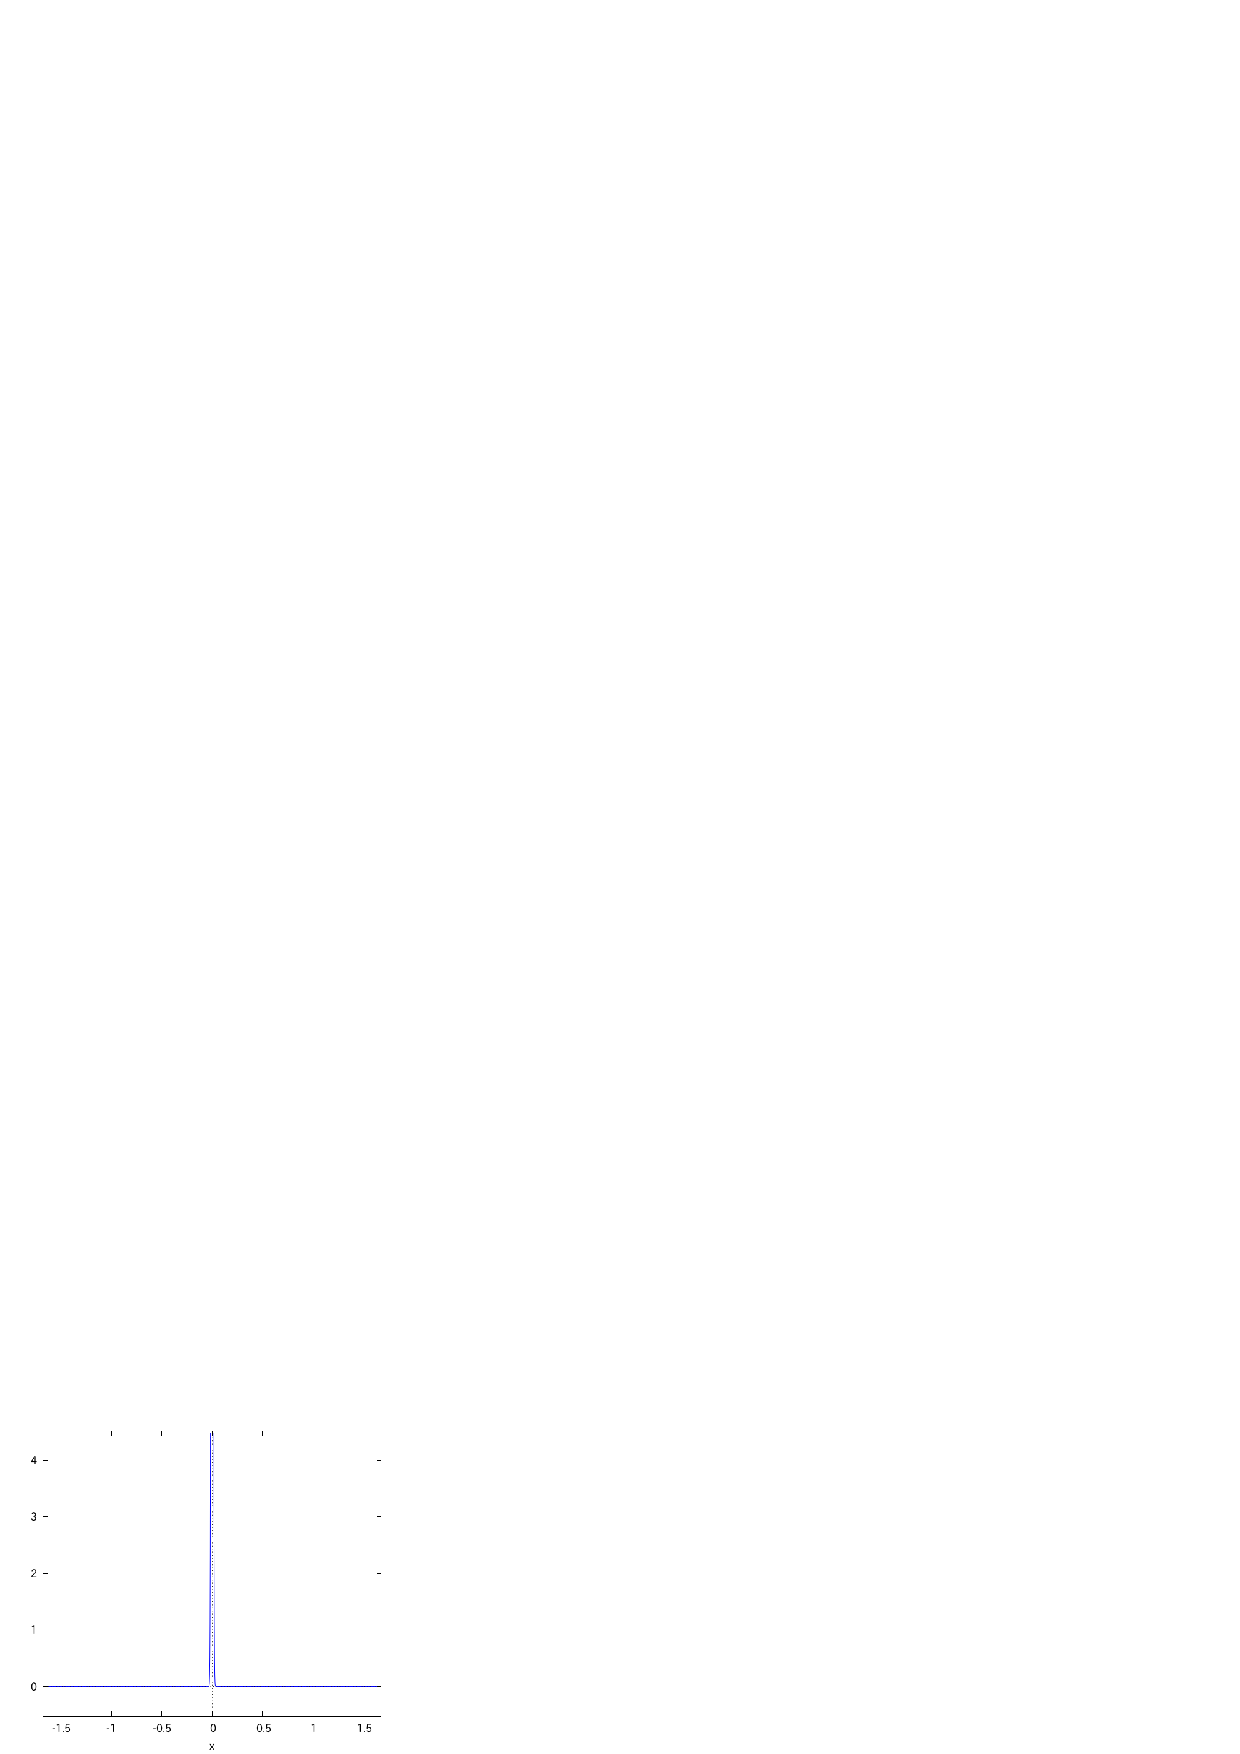
\includegraphics[keepaspectratio, width=6.5cm,height=6cm,clip]{Dirac_Delta_function3.pdf}
                        \caption{ディラックの $\delta$ 関数(1次元)の形}
                        \label{fig:delta_f2}
                    \end{center}
                \end{figure}

                        作り方は簡単.まず,面積1のグラフを用意する(図\ref{fig:delta_f24}).
                \begin{figure}[hbt]
                    \begin{center}
                        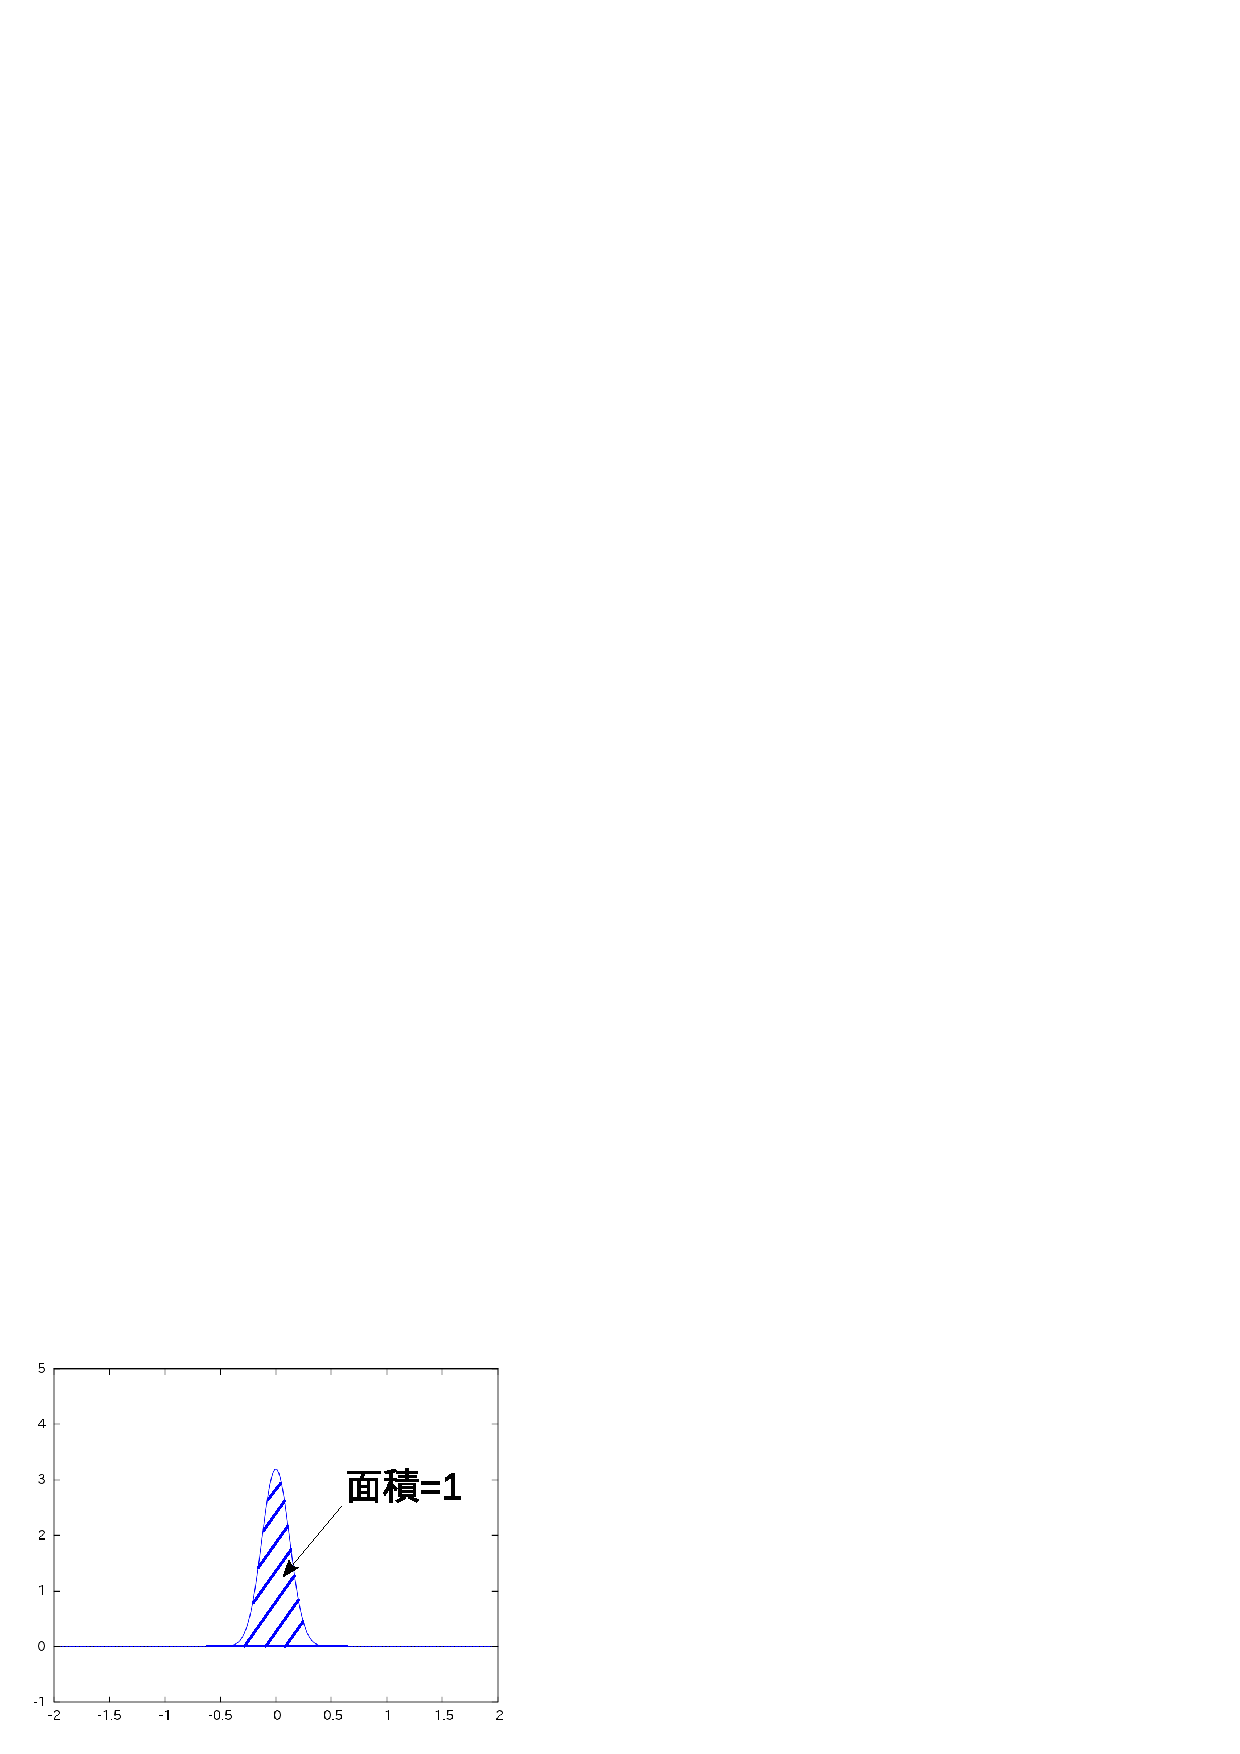
\includegraphics[keepaspectratio, width=6.5cm,height=6cm,clip]{Dirac_Delta_function5.pdf}
                        \caption{ディラックの $\delta$ 関数の作り方1}
                        \label{fig:delta_f24}
                    \end{center}
                \end{figure}

                        そして,面積1を保ちながら無限に細くしていく(図\ref{fig:delta_f33}).
                \begin{figure}[hbt]
                    \begin{center}
                        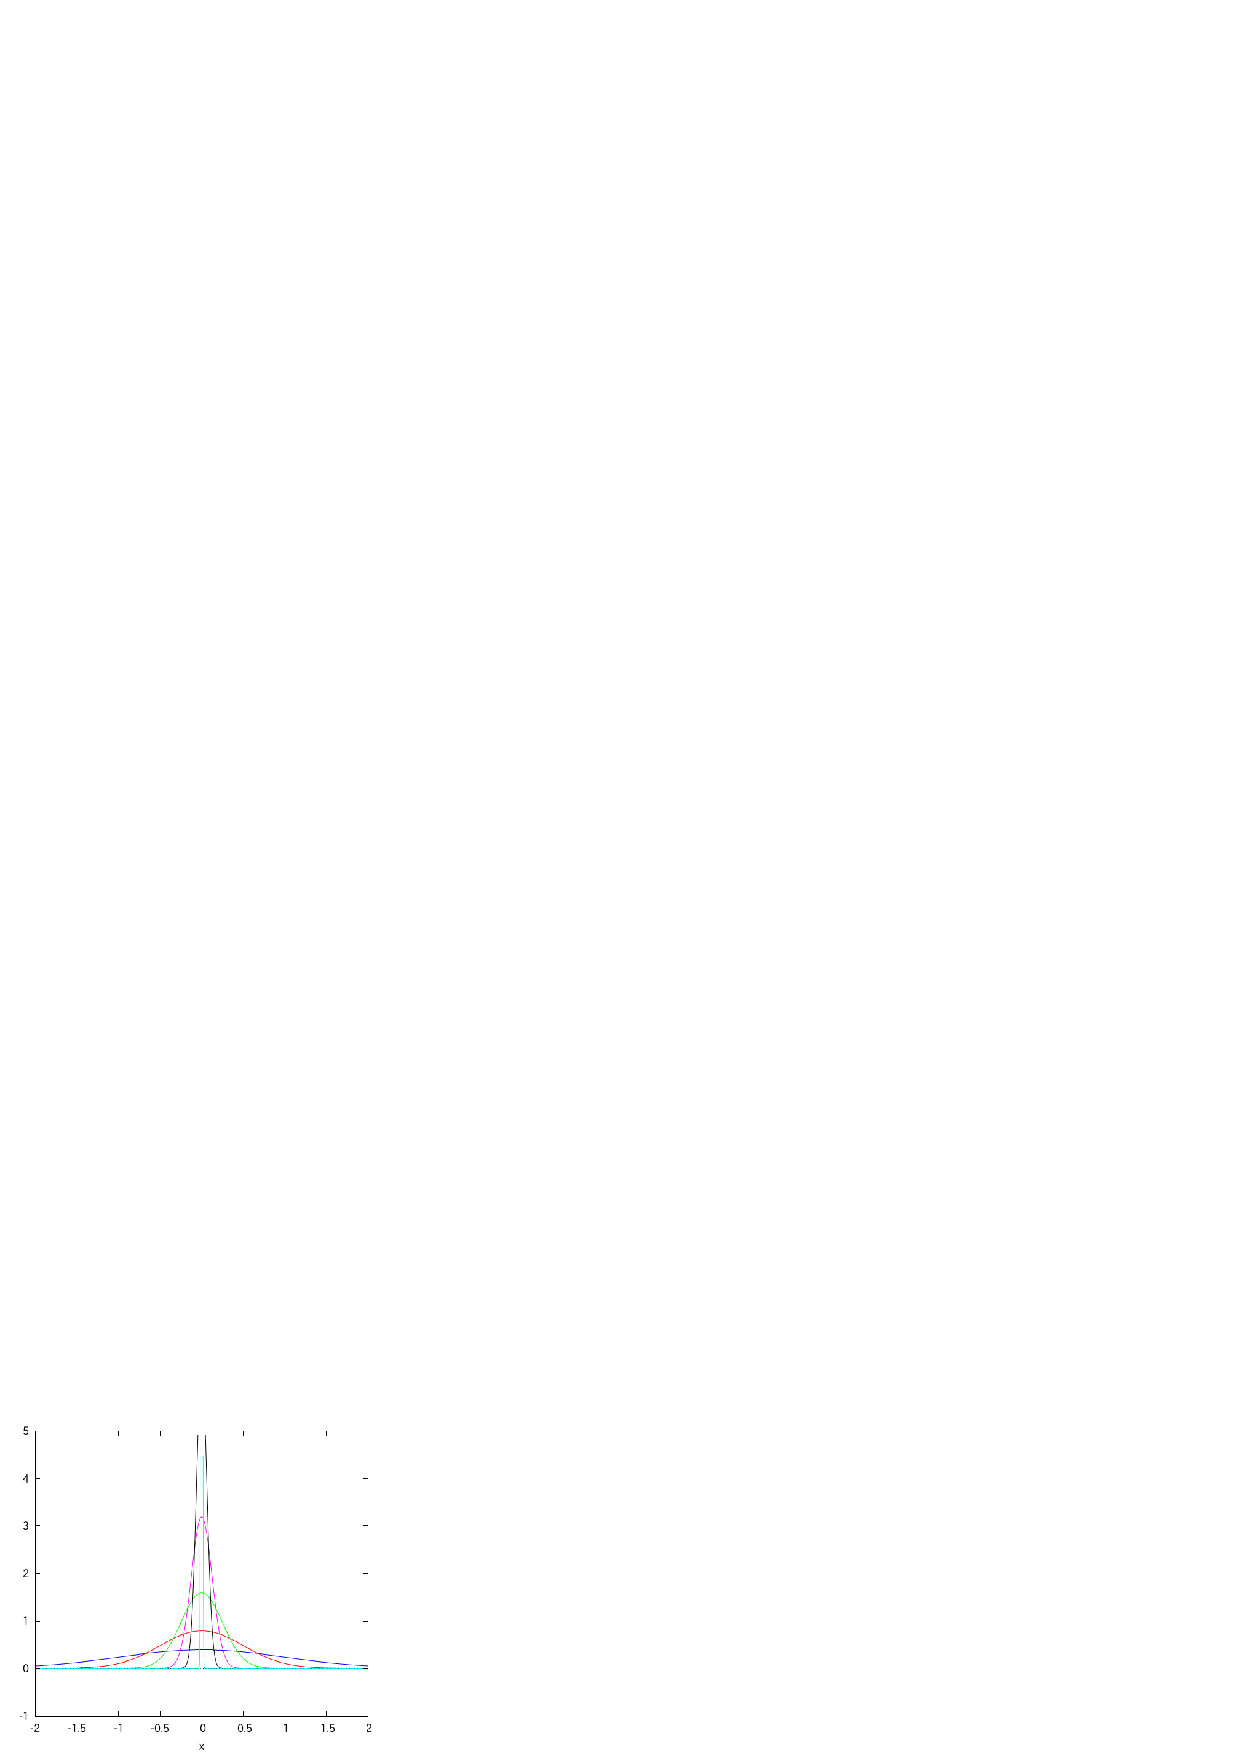
\includegraphics[keepaspectratio, width=6.5cm,height=6cm,clip]{Dirac_Delta_function4.pdf}
                        \caption{ディラックの $\delta$ 関数の作り方2}
                        \label{fig:delta_f33}
                    \end{center}
                \end{figure}
                        これで,面積が1で関数値が無限になる関数を作ることができた.

            $\delta$ 関数には次元があり,[$x^{-1}$] である.次元を持っていることを忘れやすいので,要注意.

                        ついでに,2次元の $\delta$ 関数のグラフも書いておこう.は図\ref{fig:delta_f66}下の通り.
                \begin{figure}[hbt]
                    \begin{center}
                        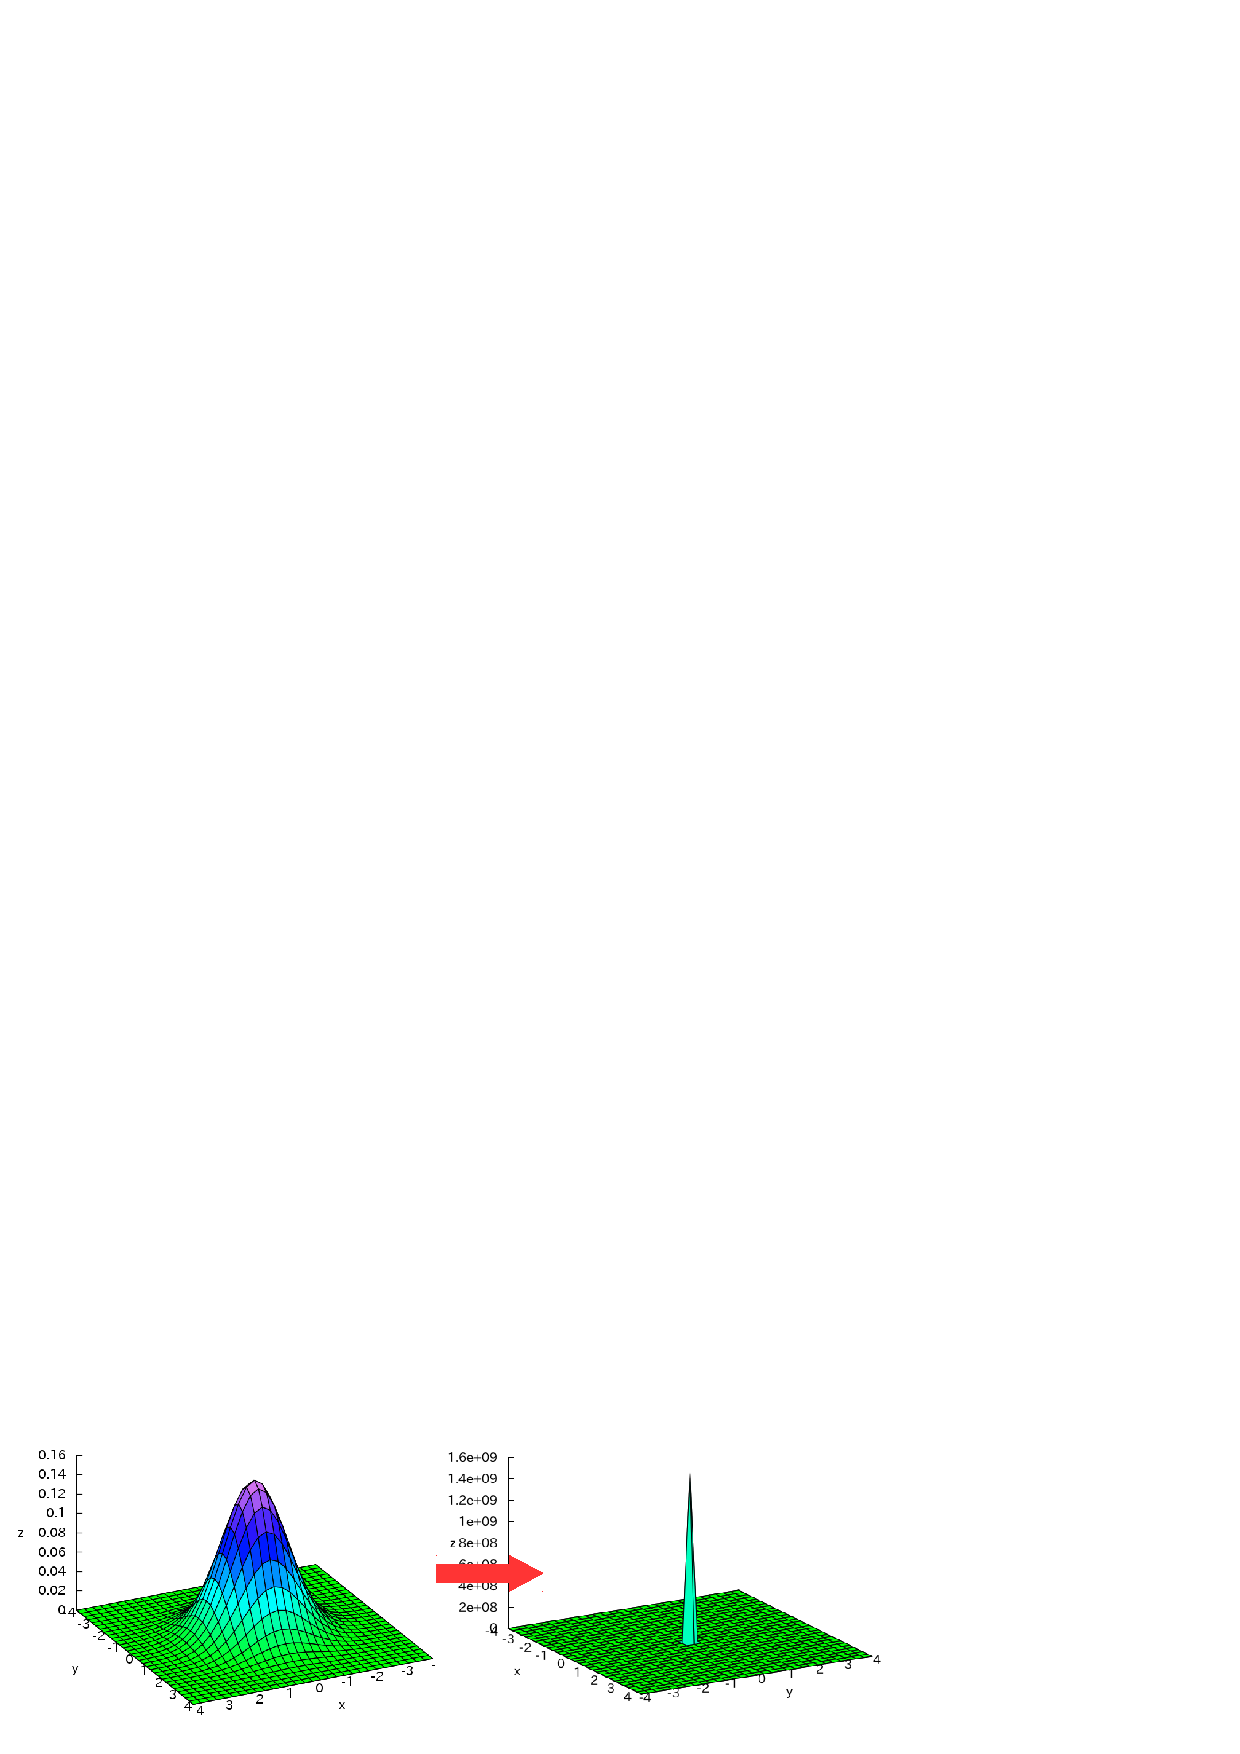
\includegraphics[keepaspectratio, width=6.5cm,height=6cm,clip]{Dirac_Delta_function6.pdf}
                        \caption{ディラックの $\delta$ 関数(2次元)の形}
                        \label{fig:delta_f66}
                    \end{center}
                \end{figure}

                        残念ながら,現実世界である3次元の $\delta$ 関数は図には描けない...

%======================================================================
%  Section
%======================================================================
\section{電流}
%======================================================================
%  SubSection
%======================================================================
    \subsection{電流のイメージ}
    おそらく,電流は説明するまでもないだろう.電気の流れのことである.い
    ままでの言葉を使えば,\textbf{電流} とは電荷の運動のことである,とい
    えよう.観測者Aに対して,荷電粒子が速度を持って運動しているとき,観測
    者Aは荷電粒子を見て,「電流が生じている」と認識するのである.この運動
    する荷電粒子は,一般に,数え切れないほど多くの数であることを想定する
    場合が多い.特に断りのない限り,電流とは,多数の荷電粒子の運動である.

    電気回路に流れる電流も多数の荷電粒子の流れであるが,この荷電粒子は導
    線中を移動することしかできない.そこでここでは,もう少し電流のイメー
    ジを拡張して,任意の空間に流れる電流を認めよう.荷電粒子は導線内部に
    しか存在できないわけではない.真空中に存在することもある.電流は導線
    だけに流れるものではない.

    電流を記号で表すときには,$I$ を用いることが多い.

    電気回路での電流のイメージは図\ref{fig:EM_Denryu01}(A)のようになろう.
    導線の中の電子をイメージしたら,図\ref{fig:EM_Denryu01}(B)の様になるかもしれない.
    しかし,実は図\ref{fig:EM_Denryu01}(B)のイメージは物性物理学的に間違っている.
    実際の電流の発生機構を説明するには原子の構造の解明や量子力学の知識が必要であり,
    それをここで考えることはできない.
    しかし,電磁気学では電荷の流れ方がどのようになっているかは説明できない.
    それとは関係なしに理論が成立している.

    電磁気学での電流とは電荷の移動であり,その場所は問われていない(導線内部である必要はない).
        具体的イメージも大事だが,ここではそれにとらわれず,抽象的な電流を考えるべきである.
        何度も言うが,電流とは空間中を移動する電荷のことである.どのように移動するかは別問題である.
        そうした抽象的な電流を考えるならば,図\ref{fig:EM_Denryu01}(B)のイメージは,
        荷電粒子の通り道を任意の空間と捉えることで,正しいイメージとなる.
        \begin{figure}[hbt]
            \begin{tabular}{cc}
                \begin{minipage}{0.5\hsize}
                    \begin{center}
                        \includegraphicsdouble{EM_Denryu01.pdf}

                        (A) 電気回路
                    \end{center}
                \end{minipage}
                \begin{minipage}{0.5\hsize}
                    \begin{center}
                        \includegraphicsdouble{EM_Denryu02.pdf}

                        (B) 一般化
                    \end{center}
                \end{minipage}
            \end{tabular}
            \caption{電流(イメージ)}
            \label{fig:EM_Denryu01}
        \end{figure}



%======================================================================
%  SubSection
%======================================================================
    \subsection{電流の定義(仮)}
        電流を数式を用いて定義しておこう.電流とは多数の点電荷の集まりの平均的な移動
        のことである.この移動を畏まった言い方をすると,次のように言える.

        ここに電流の通り道(導線)があるとしよう.
        このとき,電流を次のように定義する.
        \\
        \begin{itembox}[l]{\textbf{電流の定義(仮)}}
            \begin{itemize}
                \item 電流とは,導線の断面を単位時間1[s]に通過する
                      電荷の量を,\textbf{電流} という
                \item 電流の単位は[A]という記号で表される
                \item 電荷の単位はクーロン([C])であるので,電流の単位[A]は
                      [A]$=$[C/s]という関係がある
                \item 電流を表す標準的な記号として,このノートでは,$I$,
                      もしくは,$i$ を用いることにする
                        \footnote{
                            記号 $i$ は数学では虚数単位として用いられる
                            記号であるが,物理学や工学では電流を表すことに
                            用いることが多い(その方が一般的).なので,
                            物理学では虚数単位として,$j$ が採用されている.
                            $i$ の次のアルファベットだからだろうか.おそらく,
                            特別の意味などはないはず.文字の意味に注意しよう.
                        }
            \end{itemize}
        \end{itembox}
        \\
        \begin{figure}[hbt]
            \begin{center}
                \includegraphicslarge{EM_Denryu.pdf}
                \caption{電流(イメージ)}
                \label{fig:EM_Denryu}
            \end{center}
        \end{figure}

    \begin{memo}{注意}
        実は,この電流の単位は現在では採用されていない.
        正式な単位の定義は,後に必要な知識を説明した上で行う.
        電流に単位がないと,電流に関する事柄を扱いにくいので,
        ここではとりあえず,最も直感的で自然な定義を説明した.
        この節で「(仮)」と表現しているのは,このことによる.
    \end{memo}

%======================================================================
%  SubSection
%======================================================================
    \subsection{電流密度}
    電流とは,導線の垂直断面を,一秒間に流れる電気量として定義した.
    さらにここで,単位断面積1[m${}^{2}$]を単位時間1[s]の間に,
    どのくらいの電流が生じるかを示す \textbf{電流密度} を定義する
        \footnote{
            注意しておこう.電流密度の“密度”とは,単位面積当たりの
            密度のことである.電荷密度では,単位体積当たりの密度のこ
            とであり,両者(電荷密度と電流密度)の“密度”という語彙
            の違いは区別しておく必要がある.(次元解析をしていて,これ
            らの単位を混同してしまって,頭が混乱してしまったことがあ
            る.時間の無駄であった.)
        }.

        導線に生じている電流 $I$ が,いかなる場合でも,一様で
            \footnote{
                一様に:“むらなく”とか,“偏りなく”といった意味で使用される語彙.
            }
        あるならば,電流密度を導入することは無駄である.しかし,
        現実には,導線に生じる電流は一様ではなく,ある部分に集中的に多く
        流れていたり,ある部分には電荷の流れが全くないこともある.たしかに
        導線全体を見渡した正味の電流は一定値をとっているが,その導線の内部
        を詳細に見ることができるならば,電流にむらがあることを知るだろう.

        電流密度を $\bi(\br)$ と表す.単位は[A/m${}^{2}$]である
            \footnote{
                電荷密度 $\rho$ の単位 [C/m${}^{3}$]との違いに注意.
                電流密度は単位面積当たりの量で,電荷密度は単位体積当たり
                の量である.
            }.
        \begin{figure}[hbt]
            \begin{center}
                \includegraphicslarge{EM_DenryuMitsudo1.pdf}
                \caption{電流密度(イメージ)}
                \label{fig:EM_DenryuMitsudo1}
            \end{center}
        \end{figure}

%======================================================================
%  SubSection
%======================================================================
    \subsection{電流密度と電流の関係}
        電流 $\bI$ と電流密度 $\bi$ の関係を示そう.
        まず,電流の大きさ $I=|\bI|$ と電流密度 $\bi(\br)$ の関係を考える.

        導線の断面を $S_{l}$ とし,また,
        その一部の微小断面を $\df S_{l}$ とする
            \footnote{
                添字の $l$ は曲面 $S_{l}$ の縁となる閉曲線を表す.
                一般に,曲面は縁があるはずで,その縁は閉曲線である.
            }.
        この微小断面 $\df S_{l}$ の単位法線ベクトルを $\bn(\br)$ とかこう.

        このとき,電流密度 $\bi(\br)$ の微小断面 $\df S_{l}$ の垂直成分は
            \begin{align*}
                \bi(\br) \cdot \bn(\br) \df S_{l}
            \end{align*}
        で表現できる.そして,これを全断面 $S$ で面積分した値は,
        電流の大きさ $I$ に等しい.すなわち,
            \begin{align*}
                I = \sint_{S_{l}}\bi(\br) \cdot \bn(\br) \df S_{l}.
            \end{align*}

        まとめておこう.
        \begin{myshadebox}{電流密度と電流の関係}
            閉曲線 $l$ を縁とする曲面 $S_{l}$ を貫く電流 $I$ と,
            電流密度 $\bi(\br)$ の関係は,次式で表される.
            \begin{align}
                I = \sint_{S_{l}}\bi(\br) \cdot \bn(\br) \df S_{l}.
            \end{align}
            ここに,$\bn(\br)$ は $S_{l}$における各微小部分 $\df S_{l}$ の
            単位法線ベクトルである.
        \end{myshadebox}

        \begin{figure}[hbt]
            \begin{center}
                \includegraphicslarge{LI_si_00.pdf}
                \caption{電流と電流密度}
                \label{fig:LI_si_00}
            \end{center}
        \end{figure}

    \begin{memo}{微小面積と単位法線ベクトル}
        微小面積とは,全面積 $S$ の微小な一部分のことである.
        また,単位法線ベクトルとは,面に垂直方向で長さが1のベクトルのことである.
        \begin{figure}[hbt]
            \begin{center}
                \includegraphicslarge{EM_smollS.pdf}
                \caption{微小体積}
                \label{fig:EM_smollS}
            \end{center}
        \end{figure}
    \end{memo}

    \begin{memo}{面積分の表示方法}
        面積分は,2方向にわたる積分である.
        つまり,2つの積分変数 $u$,$v$ を
        考えたとき,これを変数に持つ関数 $f(u,\,v)$ をとし,
            \begin{align*}
                \int \left( \int f(u,\,v) \df u \right) \df v
            \end{align*}
        を計算することが,面積分を行うということである.

        つまり,$f(u,\,v)$ を最初に $u$ について積分して,その結果をさらに,
        $v$ について積分するということである.計算方法を示すには,このような
        表示の仕方が有効であるが,この表現からでは面積分であることをイメージする
        には,少々難しい.そこで,式を次ように書き換えてみる.
            \begin{align*}
                 \sint f(u,\,v) \df u \df v
            \end{align*}
        括弧をなくしただけである.そして,
        $\df S := \df u\df v$ という量を導入し,
        さらに,2回の積分を改て $\sint_{S}$ と表現することで,
            \begin{align*}
                \sint_{S} f(u,\,v) \df S
            \end{align*}
        となる.これならば,面 $S$ で面積分するというイメージが
        しやすい式の表現になった.

        ちなみに,$\df S := \df u\df v$ は \textbf{面積素} とよばれる.
    \end{memo}

